%%%%%%%%%%%%%%%%%%%%%%%%%%%%%%%%%%%%%%%%%%%%%%%%%%%%%%%%%%%%%%%%%
%%%%%%%%%%%%%%%%%%% Blueprint of DSynkant %%%%%%%%%%%%%%%%%%%%%%%
%%%%%%%%%%%%%%%%%%%%%%%%%%%%%%%%%%%%%%%%%%%%%%%%%%%%%%%%%%%%%%%%%

\documentclass[11pt]{report}
\usepackage[usenames]{color}
\usepackage{graphicx}

\newcommand{\question}[1]{{\color{Green}#1}}

\title{Blueprint of DSynkant\\
  \&\\
  reverse engineering of Roland D-50}

\author{Nil Geisweiller}

\begin{document}

\maketitle

\tableofcontents

\chapter{Introduction}

\section{What is this document about?}

The goal of this document is to describe in all details every missing
information from the official documentation of Roland D-50.

\section{What this document is not?}

This document is not a user manual of DSynkant. For this purpose you should 
referee to the manual of DSynkant available on the official website of
DSynkant\\
\begin{center}\texttt{http://dsynkant.sourceforge.net}\end{center}

\section{How to read this document?}

This document contains both answers and questions not answered yet.
When you see \question{green} somewhere in the document you'll know it is a question.
If you have the answer of any
question please contact me at\\
\begin{center}\texttt{a-lin{\color{Red}[try\_to\_remove\_that]}@users.sourceforge.net}
\end{center}
{\tiny if you notice english mistakes please contact me too...}

\chapter{The engine}
In this chapter it is question of the engine of the synthesizer and also
everything concerning the conversion between the parameters manipulated by
the user \emph{(user parameters)}
and the internal parameters of the engine \emph{(engine parameters)}.

\section{Notations}
\subsection{User parameters and engine parameters}
To recognize the difference
between the user parameters and the engine parameters, the user parameters
will have the post-fix \_usp added and the engine parameters
no particular notation.
\subsection{Mathematical notations}
\begin{tabular}{rl}
  $Int[n.m]$ & the set of integers between $n$ and $m$ included\\
  $Real[n, m]$ & the set of reals between $n$ and $m$ included\\
  $log(x)$ & the natural logarithm, that is the inverse function of exp(x)
\end{tabular}

\section{Wave generator}

\subsection{Wave form}
\subsubsection{Synthesizer sound generator}
\begin{itemize} 
  \item Square form~: \\
    \includegraphics{pulsewidth.eps}  \\
    The relation between
    $pulseWidth\_usp \in Int[0,100]$ and $pw\in Real[0.5,1]$ can be
    well approximated by the following equation~:
    \[pw = \gamma \times log(\alpha * pulseWidth\_usp + \beta)\]
    where $\alpha = 1.17844$, $\beta = 11.7539$ and $\gamma = 0.201171$.
    \question{Like for the sawtooth form,
      the square form seems to have a resonnance
      filter when the pitch goes higher. Filter to determine.}
  \item Sawtooth form~:\\
    The sawtooth form is describred by the following function~:
    \[st(t) = sq(t) \times cos(w\times t + \epsilon)\]
    where $sq(t)$ is the square form defined above, $w$ the
    angular frequency ($w = 2\pi\times f$) and $\epsilon$
    a slight shifting forward phase that occurs when the pitch is lower.
    \question{Determine $\epsilon$.}
    In addition there is a sligth resonnance filter when the pitch
    gets higher. \question{Filter to determine.}
\end{itemize}

\subsubsection{PCM sound generator}

\section{Chorus}
The chorus of D-50 takes in input a mono signal
and outputs a stereo signal.

\section{Miscellaneous or not yet classified}
\begin{itemize}
  \item It seems that the only stereo in a patch comes from chorus and reverb.
\end{itemize}
  

\chapter{Banks and patches}

Most of the information is well detailed in the documentation of VC-1 so
for the moment I see no open question about banks and patches format.

\chapter{Acknowledgements}
Below is the list of all people that helped me making this document~:\\

\begin{tabular}{ll}
Frank Neumann
&
\end{tabular}

\end{document}
